\documentclass{article}
\usepackage{graphicx} % Required for inserting images
\usepackage[square,numbers]{natbib}
%\usepackage{natbib}
\bibliographystyle{unsrtnat}
% \usepackage[
% backend=biber,
% style=alphabetic,
% sorting=ynt
% ]{biblatex}

%\addbibresource{mybib.bib}

\title{Case Study on Ethical Issues of Using Blockchain and NFT Technology for Digital Trade Sales}
\author{Sama Samrin, ID: 1191609}
\date{May 24, 2023}

\begin{document}

\maketitle

\section{Abstract}
Built on blockchain technology, Non-fungible Tokens (NFTs) have risen in popularity since 2021 as a unique medium of purchasing or trading digital art using cryptocurrencies like Ethereum. Although it provides a viable alternative for modern artists to have digital ownership of their authentic creations and earn from them via features like royalty agreements, it simultaneously impacts the environment adversely and operates on problematic regulations. The relevant issues cover a wide spectrum including stolen art, untested smart contracts, influencer scams and more. In this study, we will take a deeper look at how the NFT technology and its regulatory vulnerabilities have been exploited by malicious individuals to implement fraudulent schemes, money laundering and similar criminal activities.
\\\textit{\textbf{Index Terms-}} Ethics, Blockchain, NFTs, Ethereum.

\section{Introduction}
Blockchain technology allows peer-to-peer monetary transactions between participants existing on the same network. These transactions are then approved by consensus and recorded on a digital decentralized ledger, which is accessible from each participant’s device. Each party gets two kinds of digital keys - public (which can be shared with anyone) and private (which must be kept secret). This entire blockchain architecture and technology is the backbone and source of power for NFTs.

NFT or Non-fungible Token is a unique cryptographic representation of ownership for digital, virtual and occasionally physical assets. Professor Michael Dowling \cite{DOWLING2022102097} defines NFTs as “tradeable rights to digital assets (images, music, videos, virtual creations) where ownership is recorded in smart contracts on a blockchain”. Even though it gained popularity in this decade, the first ever NFT was a video clip tokenized by Kevin McKoy in 2014. \cite{9803425}

Since then, both NFT space and cryptocurrency universe have undergone many changes and achieved numerous milestones.  On one hand, NFT is considered to be a strong solution for patent protection \cite{barakat2022use}, digital copyright issues \cite{Rafli_2022} and low profit share of artists \cite{Chainalysis}. On the other hand, with more sets of eyes on such activities, there has also been an increase in malicious intruders finding loopholes in blockchain technology to satisfy their greed. Determining the causes, types and solutions to these issues is extremely important for ensuring  the safety of current and future groups of artists, traders and crypto experts.

\section{Fundamentals of NFT Technology}
The term ‘fungible’ is typically used to represent inherently valuable items that can be exchanged with other items of the same category. For instance, common money or notes of the same currency is a fungible item, because it has intrinsic value and you can exchange a C$20 note for two C$10 notes. Similarly, cryptocurrencies residing on the same blockchain are interchangeable and they can be exchanged for fiat currencies as well (such as GBP, Euro and Chinese Yuan). \cite{UMAR2021121025}

Unlike them, NFTs are non-fungible tokens because they are not interchangeable even when they are on the same blockchain. \cite{Investopedia} They can be traded for other NFTs but not substituted.

New NFTs are generated through the minting process where their unique information is recorded on a newly created block of the blockchain and then verified by a validator. To ensure the safety of transactions and ownership transfers, every NFT needs to follow standards like ERC-721 or ERC-1155. \cite{9803425} Minting also allows the creator to set the price, rules and royalties for the NFT \cite{10.1145/3474355} in the corresponding encoded smart contract.

The digital agreements called smart contracts are basically computer programs embedded within the blockchain. Kai Peng et al \cite{9409120} define it as “a decentralized program with a set of self-enforcing agreements on the blockchain”. Unlike regular contracts, a smart contract is immutable and distributed, i.e. no one can change it after creation and everyone on the network needs to validate it. 

\section{Ethical Challenges of NFT Trades}
NFT primarily garnered popularity in the public eye in mid-2021. According to the annual Crypto Crime Report published by Chainalysis \cite{Chainalysis}, the amount of cryptocurrency sent to Ethereum-based smart contracts increased from \$106 million in 2020 to at least \$44.2 billion in 2021.[Figure 1]

\begin{figure}[ht]
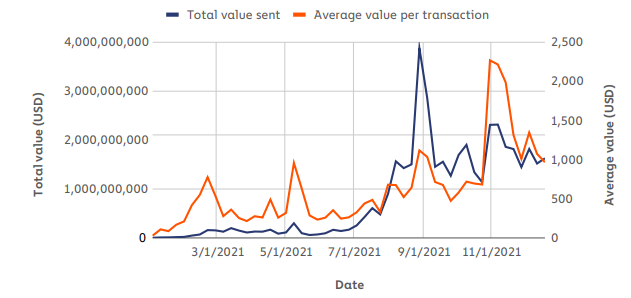
\includegraphics[width=12cm]{fig}
\caption{Weekly total cryptocurrency value and average value per transaction sent to NFT platforms throughout 2021, Chainalysis Cyber Crime Report 2022}
\end{figure}

This lucrative market of NFTs has led to a number of ethical and criminal issues such as wash trading, money laundering, fraudulent products and hacking. 

\subsection{Wash Trading}
Wash trading occurs when the seller himself purchases his NFT in order to increase its market value and trading volume artificially. This leads potential buyers to perceive its inflated cost as reality and they end up investing more money on this product than its actual worth. In 2022, Von Wachter et al conducted an analysis \cite{vonwachter2022nft} on 52 of the largest NFT collections and observed around 4\% of addresses processed over 2\% of all the sales. Such suspicious transactions may have inflated the relevant trading volumes by about \$150 million between 2018 and 2021.

Such occurrences are common within the NFT universe because the trading platforms like OpenSea only ask for the user’s cryptocurrency wallet and the associated private key to open an account, without any other personal authorization requirement. So the same individual can own multiple cryptocurrency wallets and then connect them to separate accounts. Then they use one of these accounts to buy their own NFT from another account to increase its value to actual buyers. This also increases its trading volume which is another factor most high-quality investors look for. 

\subsection{Money Laundering}
The wash trading mechanism is also used for money laundering purposes. In this case, the launderer can buy an NFT from another account he owns or sell it to a trusted third party involved in the same criminal network. \cite{treasurydepartment} This creates a sales record which then they can show as a legitimate source of earnings.

\subsection{Scams}
Additionally, there have been numerous NFT scams where an influencer or a fraudster tricks unsuspecting people (with little knowledge of cryptocurrency) to purchase NFTs at a much higher price than their worth. Another form of scam is where fake NFTs resembling real notable collector NFTs are sold to the victims.

Utilizing their impact on social media and the gullibility of their audience, certain online personalities have caused many of their followers to fall for NFT scams and earn huge figures for their own crypto wallets. Using the virality of such content as a factor, Sayak Saha Roy et al \cite{roy2023demystifying} conducted a study analyzing 439 Twitter accounts that scammed people with over a thousand NFT phishing attacks and fake giveaway competitions of NFT collections. 

According to Chainalysis report of 2022 \cite{Chainalysis}, scammers have garnered the highest profits from the countries of Canada, the USA and Australia.

\begin{figure}
    \centering
    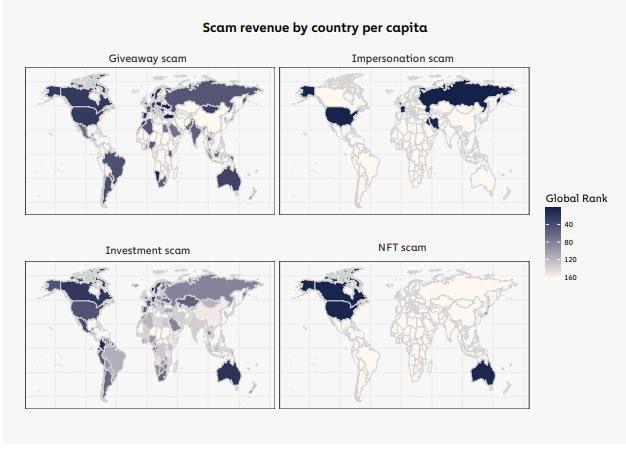
\includegraphics[width=12cm]{scam_2022.png}
    \caption{Scam Revenue by country per capita, Chainalysis Cyber Crime Report 2022}
    \label{fig:my_label}
\end{figure}

\subsection{Hacking}
Similar to the traditional hacking of computer systems and individual identities, NFTs and NFT accounts can also be hacked by cybercriminals. These attackers target legitimate users and owners of NFTs during the minting or selling phase. \cite{wang2021non} They take advantage of authentication loopholes present in the smart contract to impersonate the user or spoof the owner’s private key to transfer the NFT’s ownership.

\section{Proposed Solutions}
Since these issues widely vary in nature, attempts to solve them also differ significantly. For instance, one way to detect and prevent wash trading is to use blockchain analysis to analyze the addresses from which the NFTs were sold. This will help us find the correlation between the buying addresses and the selling addresses. If the buying address was funded by the selling address, it can be a potential perpetrator of wash trading.

Another potential solution is to implement self-trade prevention measures which have been already implemented by traditional market exchanges. \cite{victor2021detecting} This mechanism doesn’t allow individual accounts on the publicly traded company IDEX to fill their own orders of buy or sell. 

Know Your Customer (KYC) is another common initiative implemented by such trading companies that compels users to prove their identity with official and verifiable documents. After IDEX adopted this method in 2019, the corresponding wash trading volumes in the centralized system reduced significantly. \cite{victor2021detecting}
Therefore, similar steps can be taken by the decentralized finance or DeFi ecosystem. 

Such enforced formal verification can also be imposed on users to prevent unauthorized access to NFTs and false impersonation of owner accounts. Doing so while participating in the smart contract and using cold wallets can keep their private keys secure. If the malicious individuals cannot access their private keys, it becomes substantially more difficult for them to spoof the legitimate NFT user's account and assets. As a result, the honest traders  on the platform can increase their assets while the artists can feel motivated to create more of their original pieces.

\section{Conclusion}
The whole universe of NFT, cryptocurrency and smart contracts is a relatively novel space for most of us. At the same time, it brings a wide spectrum of exciting opportunities related to art, digital assets and more. Its appeal is growing by the day due to the promises of metaverse where virtual reality and augmented reality will thrive side-by-side. We can then flaunt the NFTs we own to our peers within the metaverse bubble. These digitally unique tokens also enable artists a modern and viable way to earn from their authentic creations.

However, all of these positive scenarios can only become reality when NFT and blockchain technologies implement ethically and legally sound measures to prevent cybercrimes. Taking inspirations from traditional centralized monetary or trading systems and considering novel ideas proposed by experienced in-field researchers, the NFT world can turn into a safe space for both art and trade enthusiasts in near future.

\bibliography{mybib}
%\printbibliography
\end{document}
